\addcontentsline{toc}{section}{         **Introduction}
\section*{      **Introduction}

In the course TTK4175 - Instrumentation Systems we completed our first out of a total of 5 lab assignments, the ABB lab. Throughout this assignment, basic functions of the ABB software \textbf{ControllIT} and \textbf{Control Builder Professional 4} are presented by a "Rectangle Tutorial" and a second part consisting of testing the hardware.

The purpose of the lab is to develop a software application for the process, that is; heating water to a desirable temperature by generating power to the heater from a motor and a generator using a PID-controller. The lab is built up by several parts:

Part 1 - Rectangle Tutorial

Part 2 - Testing Hardware

Part 3 - Display for control and overview of process

Part 4 - Temperature-regulator\\

Each part is closer described in the preceding chapters.

\begin{figure}[!htb]
    \centering
    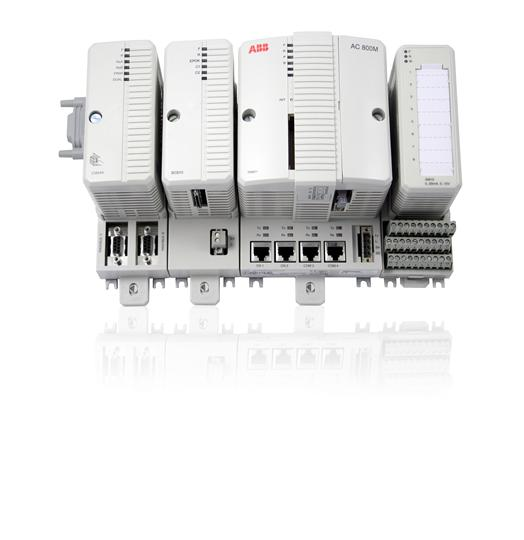
\includegraphics[width=0.8\textwidth]{images/presentation}
    \end{figure}